% ------------------------------------------------------------------------------
% TYPO3 CMS 7.1 - What's New (English Version)
%
% @author	Michael Schams <schams.net>
% @license	Creative Commons BY-NC-SA 3.0
% @link		http://typo3.org/download/release-notes/whats-new/
% @language	English
% ------------------------------------------------------------------------------
% LTXE-CHAPTER-UID:		e7264f0e-3f82290d-94c50cda-fb2d8e66
% LTXE-CHAPTER-NAME:	Backend User Interface
% ------------------------------------------------------------------------------

\section{BackendUI}
\begin{frame}[fragile]
	\frametitle{Backend User Interface}

	\begin{center}\huge{Chapter 1:}\end{center}
	\begin{center}\huge{\color{typo3darkgrey}\textbf{Backend User Interface}}\end{center}

\end{frame}

% ------------------------------------------------------------------------------
% LTXE-SLIDE-START
% LTXE-SLIDE-UID:		f9d8cbd5-57643393-2ab1a962-52d84209
% LTXE-SLIDE-ORIGIN:	d5fddde9-b3ee31c0-f0509300-40a2928e English
% LTXE-SLIDE-TITLE:		Date/Time Picker
% LTXE-SLIDE-REFERENCE:	Breaking-62925-RemoveExtJsDateTimePicker.rst
% ------------------------------------------------------------------------------

\begin{frame}[fragile]
	\frametitle{Backend User Interface}
	\framesubtitle{Look \& Feel: Date/Time Picker}

	Date/Time Picker has been replaced with a Bootstrap alternative
	\begin{figure}
		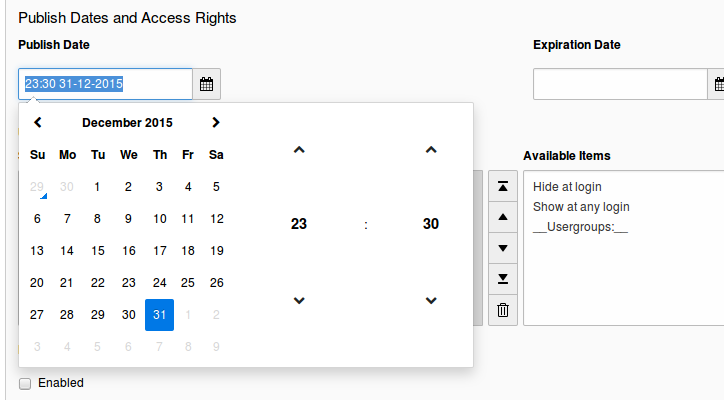
\includegraphics[width=0.75\linewidth]{BackendUserInterface/be-datepicker.png}
	\end{figure}

\end{frame}

% ------------------------------------------------------------------------------
% LTXE-SLIDE-START
% LTXE-SLIDE-UID:		8c0ca3a5-026c8f40-bdbaec2b-6cc97d25
% LTXE-SLIDE-ORIGIN:	1c391eec-dfb1dfa6-f783ae7a-d0b214ae English
% LTXE-SLIDE-TITLE:		Functions Module
% LTXE-SLIDE-REFERENCE:	Breaking-63310-Wizard-Modules-Moved.rst
% ------------------------------------------------------------------------------

\begin{frame}[fragile]
	\frametitle{Backend User Interface}
	\framesubtitle{Look \& Feel: Functions Module}

	"Create Pages" and "Sort Pages" moved to: \texttt{Web => Functions}\newline
	\smaller (in TYPO3 CMS < 7.1, they were located under "\texttt{Web => Functions => Wizards}")

	\begin{figure}
		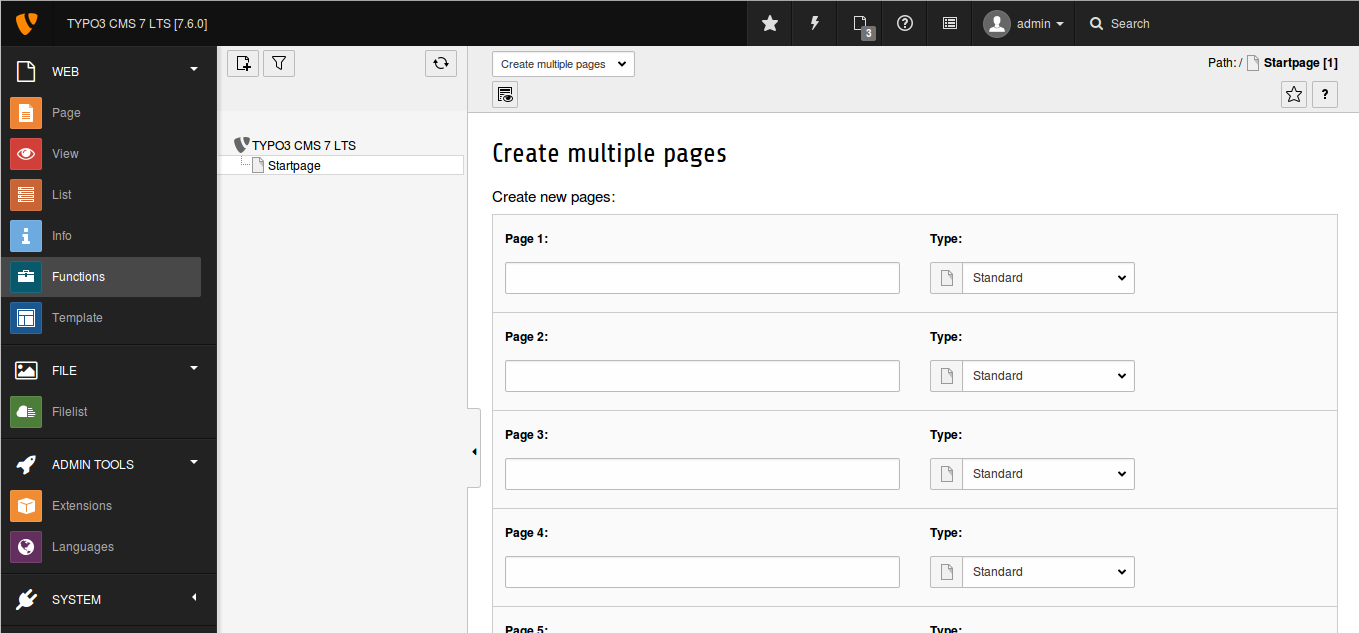
\includegraphics[width=0.80\linewidth]{BackendUserInterface/be-functions.png}
	\end{figure}


\end{frame}

% ------------------------------------------------------------------------------
% LTXE-SLIDE-START
% LTXE-SLIDE-UID:		e4722759-67f22169-8c2286ea-08c119ed
% LTXE-SLIDE-ORIGIN:	dd127630-5ccc729a-835e5836-e8796962 English
% LTXE-SLIDE-TITLE:		Access Module: Leave Unchaged
% LTXE-SLIDE-REFERENCE:	Feature-15619-LeaveUnchagedInAccessModule.rst
% ------------------------------------------------------------------------------

\begin{frame}[fragile]
	\frametitle{Backend User Interface}
	\framesubtitle{Look \& Feel: Access Module}

	Module \texttt{Web => Access} allows to leave owner/group unchanged\newline
	when overwriting permissions

	\begin{figure}
		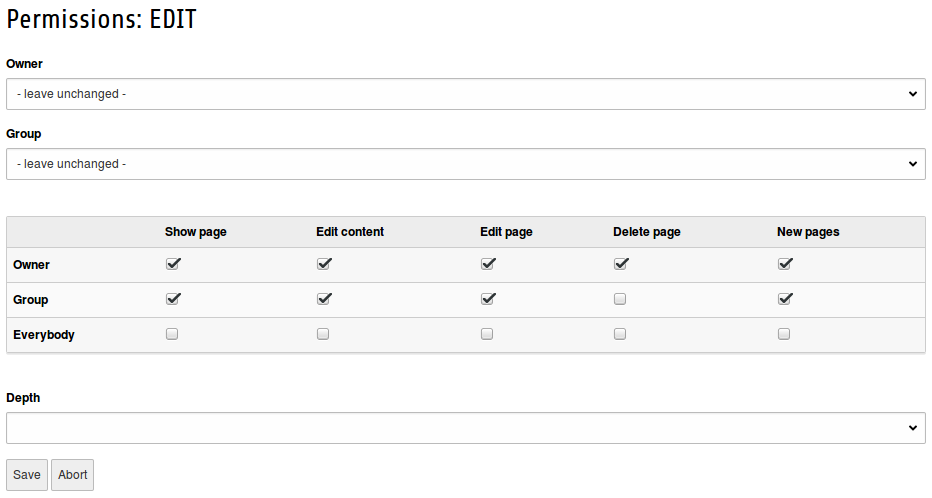
\includegraphics[width=0.75\linewidth]{BackendUserInterface/be-access.png}
	\end{figure}

\end{frame}

% ------------------------------------------------------------------------------
% LTXE-SLIDE-START
% LTXE-SLIDE-UID:		48434b48-b166fa69-849f6f0f-17aaa928
% LTXE-SLIDE-ORIGIN:	eb6cc867-e4f5d0d3-ea06672c-7ccdf227 English
% LTXE-SLIDE-TITLE:		Icons in List Module
% LTXE-SLIDE-REFERENCE:	Feature-63207-SplitActionButtonsIntoGroups.rst
% ------------------------------------------------------------------------------

\begin{frame}[fragile]
	\frametitle{Backend User Interface}
	\framesubtitle{Look \& Feel: Icons in List Module}

	Icons ("action buttons") in List module devided into two groups\newline
	\smaller (primary actions first (read, update, delete), followed by secondary actions)

	\begin{figure}
		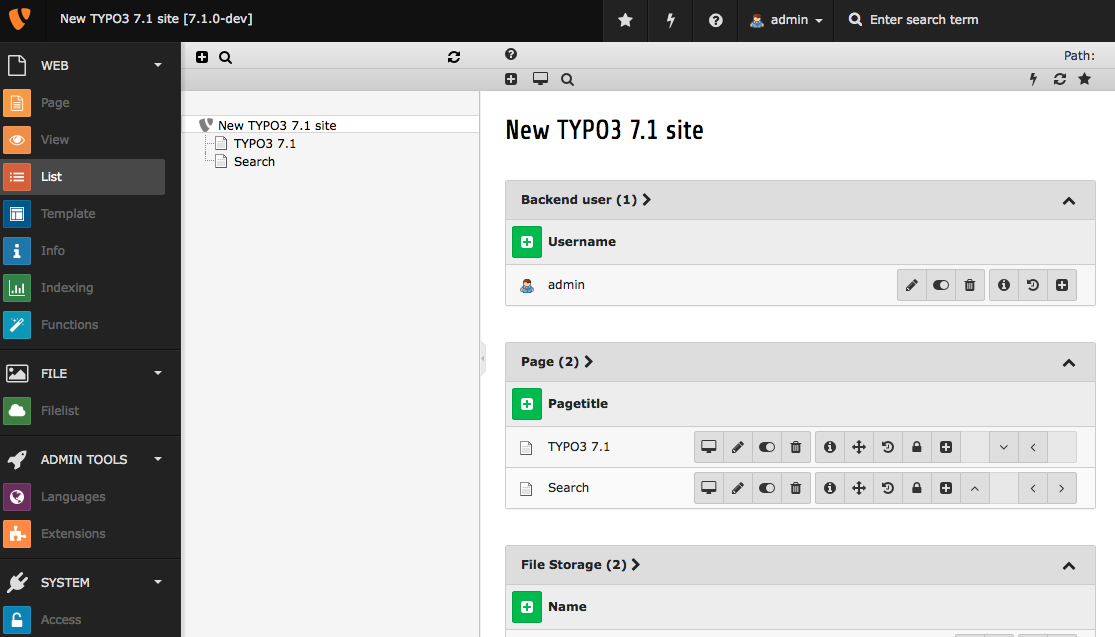
\includegraphics[width=0.75\linewidth]{BackendUserInterface/be-icons.png}
	\end{figure}

\end{frame}

% ------------------------------------------------------------------------------
